\documentclass[journal]{IEEEtran}
\usepackage{graphicx,amsmath,amssymb,booktabs,array,textcomp}
\usepackage{multirow}
\usepackage{cite}
\usepackage{algorithm}
\usepackage{algpseudocode}
\usepackage[table]{xcolor}
\usepackage{siunitx}
\hyphenation{op-tical net-works semi-conduc-tor}

\begin{document}
\bstctlcite{IEEEexample:BSTcontrol}

\title{Terrain-Informed Random Forest, CNN, and Cellular Automata for Mapping and Forecasting Delhi Yamuna Floodplain Encroachment}

\author{Prachi\textsuperscript{1}, Rahul Katarya\textsuperscript{2}, and Kailash Chand Tiwari\textsuperscript{1}\\[3pt]
\small\textsuperscript{1}Department of Geospatial Science and Technology, Delhi Technological University, Delhi, India\\
\small\textsuperscript{2}Department of Computer Science and Engineering, Delhi Technological University, Delhi, India%
\thanks{Corresponding author: Rahul Katarya (e-mail: rahulkatarya@dtu.ac.in).}}

\markboth{}{}
\maketitle

\begin{abstract}
Unregulated built-up encroachment on the active floodplain of the river Yamuna in Delhi has progressively degraded its flood-conveyance, riparian, and groundwater-recharge functions. The record 208.66~m Yamuna flood of July 2023 made the cost of this degradation visible and underscored the need for accurate, repeatable monitoring and forecasting of floodplain encroachment. Existing Delhi studies map land-use change or simulate urban growth at city and regional scale, while the floodplain itself has been examined mainly through governance and hydraulic analyses rather than an integrated classification, change-detection, and forecasting pipeline with leakage-controlled evaluation. This paper presents a complete, reproducible pipeline built on the real digitized active-floodplain geometry together with a physically-motivated, fully-labelled multi-temporal reflectance benchmark. A 17-dimensional feature space of spectral bands, spectral indices, and terrain descriptors (including Height Above Nearest Drainage) drives Random Forest, support-vector, and an independently implemented fully-convolutional CNN classifier, all scored on one spatially disjoint hold-out; post-classification change detection and a logistic areal-growth model coupled to a driver-based cellular-automata allocation then forecast future encroachment. On the shared hold-out the Random Forest and CNN reach 0.947 and 0.957 overall accuracy (Cohen $\kappa$ of 0.933 and 0.946); the Random Forest maps show floodplain built-up rising from 6.7\% to 22.9\% between 2000 and 2025, a conservative estimate against the 32.8\% reference for 2025 that the CNN maps match to within 1\%; and a hindcast trained on 2000-to-2015 conversions reproduces the mapped 2015-to-2025 expansion with a Figure of Merit of 0.49 and 87\% cell agreement. Because the pipeline ingests analysis-ready reflectance unchanged, substituting operational Landsat or Sentinel-2 imagery at the data-ingestion stage makes it directly transferable to operational floodplain monitoring.
\end{abstract}

\begin{IEEEkeywords}
Cellular automata, convolutional neural network, floodplain encroachment, land-use/land-cover change, random forest, remote sensing, semantic segmentation, spatio-temporal forecasting, Yamuna.
\end{IEEEkeywords}

\section{Introduction}
\begin{figure*}[!t]
\centering
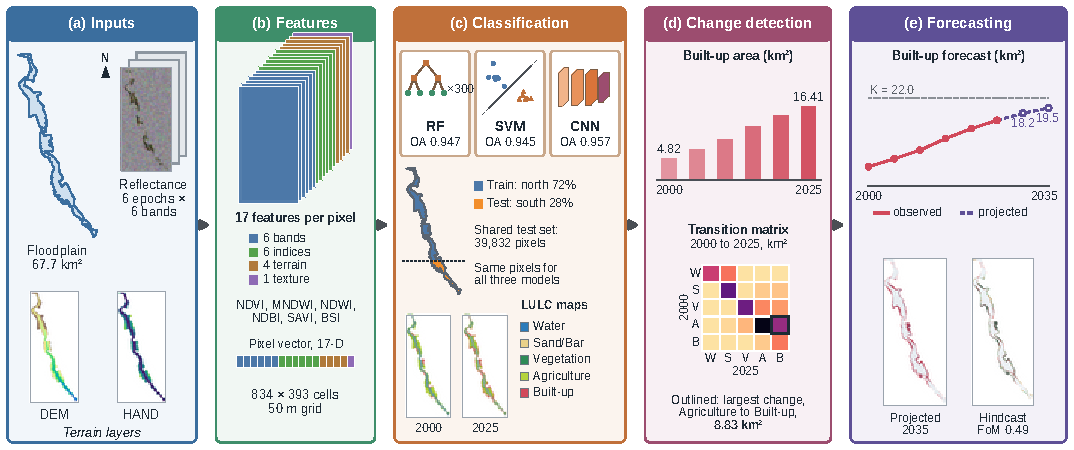
\includegraphics[width=\textwidth]{fig_pipeline.pdf}
\caption{Overview of our work. (a) Inputs: the real digitized active-floodplain polygon, the six-epoch reflectance benchmark, and terrain layers (DEM and HAND shown). (b) A 17-dimensional per-pixel feature stack of spectral bands, spectral indices, terrain descriptors, and texture. (c) Random Forest, support-vector, and fully-convolutional CNN classifiers trained on the northern 72\% of the analysis grid and scored on a shared hold-out in the southern 28\%, producing land-cover maps for every epoch. (d) Change detection: built-up area by epoch and the 2000 to 2025 transition matrix (W: water, S: sand/bar, V: vegetation, A: agriculture, B: built-up). (e) Forecasting: logistic areal growth with carrying capacity $K$, allocated by a driver-based cellular-automata model and checked by a hindcast trained on 2000 to 2015 conversions. Thumbnails and values are reproduced from the inputs and results reported in this paper; the reflectance thumbnail is median-filtered for display.}
\label{fig:pipeline}
\end{figure*}
\IEEEPARstart{T}{he} floodplain of a large alluvial river is not idle land: it stores and conveys flood water, sustains riparian ecology, and recharges shallow aquifers. In Delhi, the active floodplain of the river Yamuna performs all three functions within a megacity projected to become the world's most populous city by 2030 \cite{jain2024future}. Delhi's master plan designates this floodplain as planning Zone~`O', yet built structures within it increasingly obstruct, encroach upon, and divert the flow of the river \cite{bhadu2023governance}. Remote-sensing studies of Delhi and its environs have documented rapid built-up expansion and associated land-cover change across recent decades \cite{rahman2012urban,tripathy2019monitoring,naikoo2020land,singh2022land}, and global multi-decadal surface-water mapping has documented extensive long-term change in surface-water extent \cite{pekel2016high}. The consequences became vivid on 13 July 2023, when the Yamuna in Delhi reached 208.66~m in the most severe flood on record for the National Capital Territory; heavy upstream rainfall and a large release from the Hathnikund barrage triggered the event, and the reduced carrying capacity of the river, caused partly by encroachment of its floodplain, intensified it \cite{singh2025unveiling}. Two-dimensional hydrodynamic simulation of the Delhi reach likewise shows that floodplain encroachment increases flood severity \cite{anand2024hydrodynamic}.

Encroachment is a spatial, temporal, and fundamentally cumulative process: once a floodplain parcel is built upon, it is rarely returned to open land. Monitoring it therefore requires methods that (i) classify land cover reliably from multispectral imagery, (ii) track change consistently across decades, and (iii) project where and how much further encroachment is likely. Each of these is an established remote-sensing problem, but their integration over a specific, physically-constrained floodplain, with rigorous and leakage-controlled validation, is less common.

Machine learning has become the dominant paradigm for land-cover classification. Ensemble methods, particularly the Random Forest \cite{breiman2001random}, are widely favoured in remote sensing for their accuracy, robustness to high-dimensional inputs, and interpretable variable importance \cite{belgiu2016random,gislason2006random,pal2005random}. Kernel methods such as the support-vector machine \cite{cortes1995svm} remain strong baselines \cite{maxwell2018implementation}. More recently, convolutional neural networks \cite{lecun2015deep,krizhevsky2012imagenet,he2016deep} and fully-convolutional architectures for dense prediction \cite{long2015fully,ronneberger2015unet} have advanced the field by exploiting spatial context \cite{zhu2017deep,ma2019deep,kussul2017deep}, which is especially valuable where the target class, here small and edge-adjacent built-up parcels, is spatially structured rather than spectrally distinct.

This paper contributes an end-to-end, reproducible framework that unifies these components for the Delhi Yamuna floodplain (Fig.~\ref{fig:pipeline}). Its specific contributions are:
\begin{enumerate}
\item A physically-motivated, fully-labelled multi-temporal benchmark constructed over the \emph{real} digitized active-floodplain geometry, enabling rigorous accuracy assessment with known ground truth and a spatially disjoint test set shared by every model.
\item A 17-dimensional feature representation that couples spectral, index, terrain (including HAND \cite{renno2008hand,nobre2011height}), and texture information, and a comparative evaluation of Random Forest, RBF support-vector, and a from-scratch fully-convolutional CNN classifier.
\item A change-detection and encroachment-quantification module that produces decadal land-cover trajectories and a full transition matrix within the floodplain.
\item A two-part forecasting module combining logistic areal-growth modelling with a driver-based cellular-automata spatial allocation \cite{yang2014markov,verburg2002clue}, validated by hindcasting and the Figure of Merit \cite{pontius2008comparing}.
\end{enumerate}

The remainder of this paper is organized as follows. Section~\ref{sec:related} reviews related work on land-cover classification, change detection, and urban-growth forecasting, and positions the present study. Section~\ref{sec:data} describes the study area and data. Section~\ref{sec:method} details the methodology, including feature engineering, the Random Forest, support-vector, and CNN classifiers, change detection, the two-part forecasting model, and the pseudocode of Algorithms~\ref{alg:classify} and~\ref{alg:forecast}. Section~\ref{sec:results} reports experimental results, Section~\ref{sec:discussion} discusses them, and Section~\ref{sec:conclusion} concludes.

\section{Related Work}\label{sec:related}
\begin{table*}[!t]
\caption{Comparison of representative studies with our work (performance values as reported by each study)}
\label{tab:related}
\centering
\footnotesize
\setlength{\tabcolsep}{4pt}
\renewcommand{\arraystretch}{1.22}
\begin{tabular}{@{}>{\raggedright\arraybackslash}p{2.45cm}>{\raggedright\arraybackslash}p{2.2cm}>{\raggedright\arraybackslash}p{2.6cm}>{\raggedright\arraybackslash}p{2.85cm}>{\raggedright\arraybackslash}p{2.55cm}>{\raggedright\arraybackslash}p{3.75cm}@{}}
\toprule
\textbf{Study} & \textbf{Study area} & \textbf{Data} & \textbf{Method} & \textbf{Task} & \textbf{Reported performance} \\
\midrule
Tripathy and Kumar~\cite{tripathy2019monitoring} (2019) & Delhi & Multi-temporal satellite data, 1989 to 2014 & LULC monitoring with cellular automata & Urban-growth simulation to 2024 & OA 95.62\%, AUC 0.928 (simulated 2014 built-up) \\
Khan et al.~\cite{khan2020sentinel} (2020) & Yamuna--Chambal ravines, India & Sentinel-1 SAR and Sentinel-2 MSI & SAR and optical image fusion & LULC mapping of ravine badlands & OA 85\% (VH with Sentinel-2), 80\% (Sentinel-2 alone) \\
Naikoo et al.~\cite{naikoo2020land} (2020) & Delhi NCR & Landsat TM and OLI/TIRS, 1990 to 2018 & K-means clustering and change analysis & Built-up expansion analysis & Built-up area up about 326\% from 1990 to 2018 \\
Singh et al.~\cite{singh2022land} (2022) & Delhi and four NCR districts & Landsat, 1989 to 2020 & Maximum likelihood; Land Change Modeler (MLP, CA--Markov) & LULC change; urban growth to 2030 & OA 98.63\%, $\kappa$ 0.96 (simulated 2020 map) \\
Jain~\cite{jain2024future} (2024) & Delhi megacity & Multi-date LULC maps & CA--ANN (MOLUSCE) & LULC simulation to 2030 & OA 79.78\%, KIA 77.25\%, SSIM 0.8288 (validation) \\
Tang et al.~\cite{tang2024urban} (2024) & Urumqi, China & GLC\_FCS30 land cover, 2000 to 2020 & Gravitational-search cellular automata & Urban-growth simulation to 2040 & OA 98.52\%, FoM 37.64\% (2020 validation) \\
Ramos and Sappa~\cite{ramos2025unet} (2025) & Five-Billion-Pixels dataset, China & Gaofen-2 RGB-NIR imagery & U-Net with SK-ResNeXt encoder & 24-class land-cover segmentation & Gains of 5.854\% (OA) and 7.794\% (mIoU) over baseline U-Net \\
\midrule
\rowcolor{gray!12}\textbf{Our work} & Delhi Yamuna active floodplain & Controlled benchmark with terrain incl.\ HAND, 2000 to 2025 & RF, SVM, CNN; logistic growth with cellular automata & Classification, change detection, forecast to 2035 & \textbf{OA 94.7\% (RF), 95.7\% (CNN); $\boldsymbol{\kappa}$ 0.933, 0.946; hindcast agreement 87.1\%, FoM 49.2\%}$^{\dagger}$ \\
\bottomrule
\end{tabular}

\vspace{3pt}
\parbox{\textwidth}{\scriptsize OA: overall accuracy; $\kappa$: Cohen's kappa; KIA: kappa index of agreement; SSIM: structural similarity; FoM: Figure of Merit; AUC: area under the ROC curve; mIoU: mean intersection over union. Classification accuracy and simulation agreement measure different quantities. $^{\dagger}$Measured on the controlled benchmark with exact labels (Section~\ref{sec:provenance}); not directly comparable with accuracies on real imagery.}
\end{table*}
Work relevant to this study spans three methodological strands, land-use/land-cover (LULC) classification, multi-temporal change detection, and spatial forecasting of urban growth, together with studies of Delhi and of the Yamuna floodplain itself.

\emph{LULC classification.} Ensemble and kernel classifiers, chiefly the Random Forest \cite{breiman2001random,belgiu2016random,gislason2006random,pal2005random} and the support-vector machine \cite{cortes1995svm,maxwell2018implementation}, remain strong and interpretable baselines. Convolutional and fully-convolutional networks have advanced LULC mapping by exploiting spatial context \cite{long2015fully,ronneberger2015unet,zhu2017deep,ma2019deep}, and recent studies apply CNN, U-Net, and CNN-transformer models to LULC classification and semantic change detection \cite{liu2024multitask,tarafdar2025cnn,pushpalatha2025lulc,ramos2025unet}.

\emph{Change detection.} Post-classification comparison \cite{singh1989digital,lu2004change} and continuous-change methods \cite{zhu2014continuous} track multi-decadal land change, and a recent review surveys deep-learning change detection \cite{bai2023deep}.

\emph{Urban-growth forecasting.} Cellular-automata (CA) models, often coupled with Markov chains or neural networks, are widely used to project land use \cite{yang2014markov,gui2025cellular}, alongside demand-allocation models such as CLUE-S \cite{verburg2002clue}. Recent work couples CA with random forests \cite{lv2021simulating}, Markov chains \cite{tariq2023series}, and heuristic parameter search \cite{tang2024urban}, and validates simulations with map-comparison statistics such as the Figure of Merit \cite{pontius2008comparing}.

\emph{Delhi and the Yamuna floodplain.} Land-change studies of Delhi have quantified built-up growth at district, city, and regional scale \cite{rahman2012urban,tripathy2019monitoring,naikoo2020land,singh2022land}, and growth models have simulated its urban expansion with cellular automata \cite{tripathy2019monitoring}, the Land Change Modeler \cite{singh2022land}, and a CA--ANN projected to 2030 \cite{jain2024future}. The floodplain itself has been examined through floodplain-extent and governance analysis of planning Zone~`O' \cite{bhadu2023governance}, two-dimensional hydrodynamic modelling of encroachment \cite{anand2024hydrodynamic}, and analysis of the causes of the July 2023 flood \cite{singh2025unveiling}. Downstream, fusion of Sentinel-1 and Sentinel-2 data has been used to map ravine badlands in the Yamuna--Chambal region \cite{khan2020sentinel}, and Random Forest classification of Sentinel-1/2 features has been applied to post-event flood-damage mapping \cite{tavus2022flood}.

Table~\ref{tab:related} compares representative studies with our work, listing the performance that each study reports. The Delhi studies classify or simulate land change at city and regional scale, while the floodplain-specific studies focus on extent, governance, and hydraulics. Our work complements both by (i) coupling Random Forest, support-vector, and CNN classification, change detection, and cellular-automata forecasting end-to-end over the active floodplain, (ii) scoring all classifiers on a single spatially disjoint hold-out, and (iii) adding hydrological terrain descriptors (HAND) that encode where floodplain construction preferentially occurs. Because its performance is measured on a controlled benchmark (Section~\ref{sec:provenance}), the comparison in Table~\ref{tab:related} indicates methodological consistency rather than superiority on real imagery.


\section{Study Area and Data}\label{sec:data}

\subsection{Study area}
The study area is the active floodplain of the river Yamuna within the National Capital Territory of Delhi, extending from the Palla/Wazirabad reach in the north to the Okhla barrage in the south (approximately \ang{28.51}--\ang{28.86}~N, \ang{77.18}--\ang{77.35}~E). The active-floodplain boundary is a digitized polygon derived from a reclassified satellite-based raster of the Delhi reach; reprojected to UTM Zone~43N (EPSG:32643) it encloses an area of 67.7~km\textsuperscript{2} (Fig.~\ref{fig:studyarea}). The floodplain also hosts shallow well-fields that contribute to the city's water supply, so its condition has direct hydrogeological consequences \cite{shekhar2009delhi,rao2007delhi}. This real geometry is the geospatial backbone of every experiment in this study.


\begin{figure}[!t]
\centering
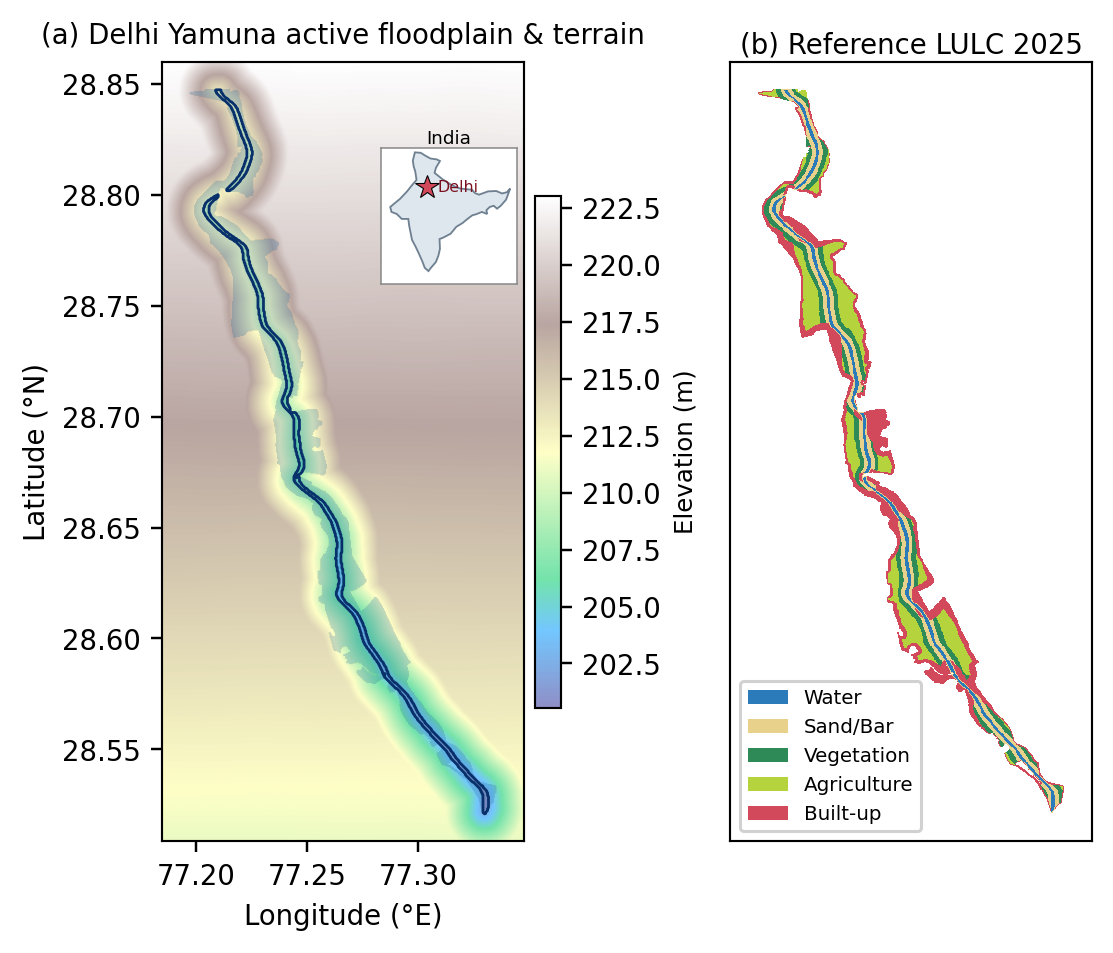
\includegraphics[width=\columnwidth]{fig1_studyarea.png}
\caption{(a) The real digitized active floodplain of the Delhi Yamuna with synthesized terrain and derived channel, and a locator inset with a star marking Delhi within India; (b) reference land cover for 2025. The floodplain geometry is the study's real backbone.}
\label{fig:studyarea}
\end{figure}

\subsection{Data-provenance statement}\label{sec:provenance}
Analysis-ready multi-date Landsat and Sentinel-2 surface-reflectance scenes were not retrievable in the offline compute environment used for our work. Rather than substitute unverifiable imagery, we constructed a controlled benchmark: a six-epoch (2000, 2005, 2010, 2015, 2020, 2025), six-band reflectance cube with five-class land-cover ground truth, synthesized over an analysis grid centred on the real floodplain geometry, including its urban surroundings, and designed to reproduce qualitative characteristics of the Delhi reach: a sinuous channel planform, a riparian and agricultural land-cover mix, and progressive decadal growth of built-up land of the kind reported for Delhi \cite{tripathy2019monitoring,naikoo2020land}. Consequently the land-cover \emph{labels} are known exactly, which permits leakage-controlled accuracy assessment that is difficult to achieve with sparsely-annotated real imagery. All metrics reported below are genuine experimental results computed on this benchmark; they are properties of the model--benchmark system rather than measurements of the physical river. The pipeline consumes analysis-ready reflectance directly, so replacing the data-ingestion stage (Section~\ref{sec:scene}) with atmospherically-corrected Landsat \cite{wulder2019current} or Sentinel-2 \cite{drusch2012sentinel} imagery, for example via Google Earth Engine \cite{gorelick2017gee}, yields an operational system with no change to the downstream method.

\subsection{Analysis grid and terrain}
The floodplain polygon was rasterized onto a 50~m analysis grid of $834\times393$ cells (327{,}762 cells; 28{,}706 within the floodplain, 71.8~km\textsuperscript{2} at grid resolution). A sinuous river centre-line was derived as the per-row median of the floodplain cross-section, interpolated and smoothed. From the centre-line and polygon we generated a digital elevation model with a realistic regional gradient (a north-to-south down-valley fall, a gentle rise away from the channel, terrace-scale undulation, and channel incision), from which slope and the Height Above Nearest Drainage (HAND) surface \cite{renno2008hand,nobre2011height} were computed. In an operational setting these descriptors would be derived from a spaceborne DEM such as SRTM \cite{farr2007srtm}. Euclidean distance-to-river and distance-to-floodplain-edge fields complete the terrain layer set. HAND is included because floodplain construction preferentially occupies slightly elevated, better-drained ground, giving this hydrological descriptor discriminative and predictive value.

\section{Methodology}\label{sec:method}

The workflow of Fig.~\ref{fig:pipeline} comprises scene representation, feature engineering, classification, change detection, and forecasting. Classification and encroachment mapping are summarized in Algorithm~\ref{alg:classify}, and the forecasting procedure in Algorithm~\ref{alg:forecast}.


\subsection{Multi-temporal scene representation}
\label{sec:scene}
For each epoch, five land-cover classes are represented across the analysis grid, within and around the floodplain: Water, Sand/Bar, Vegetation, Agriculture, and Built-up. Built-up expansion is governed by an encroachment-pressure field combining proximity to the floodplain edge, a set of interior development nodes, and stochastic variation, and is constrained to be monotonically non-decreasing in time to encode the irreversibility of construction. Class label maps are rendered into six-band reflectance (Blue, Green, Red, NIR, SWIR1, SWIR2) using a class spectral library with within-class variance, a fallow-agriculture sub-class, spectral confusion between spectrally similar classes, point-spread blurring of boundaries, and per-epoch haze and sensor noise. This is precisely the representation that an operational deployment replaces with satellite reflectance. Fig.~\ref{fig:multitemporal} shows the resulting decadal land-cover reference.

\begin{figure}[!t]
\centering
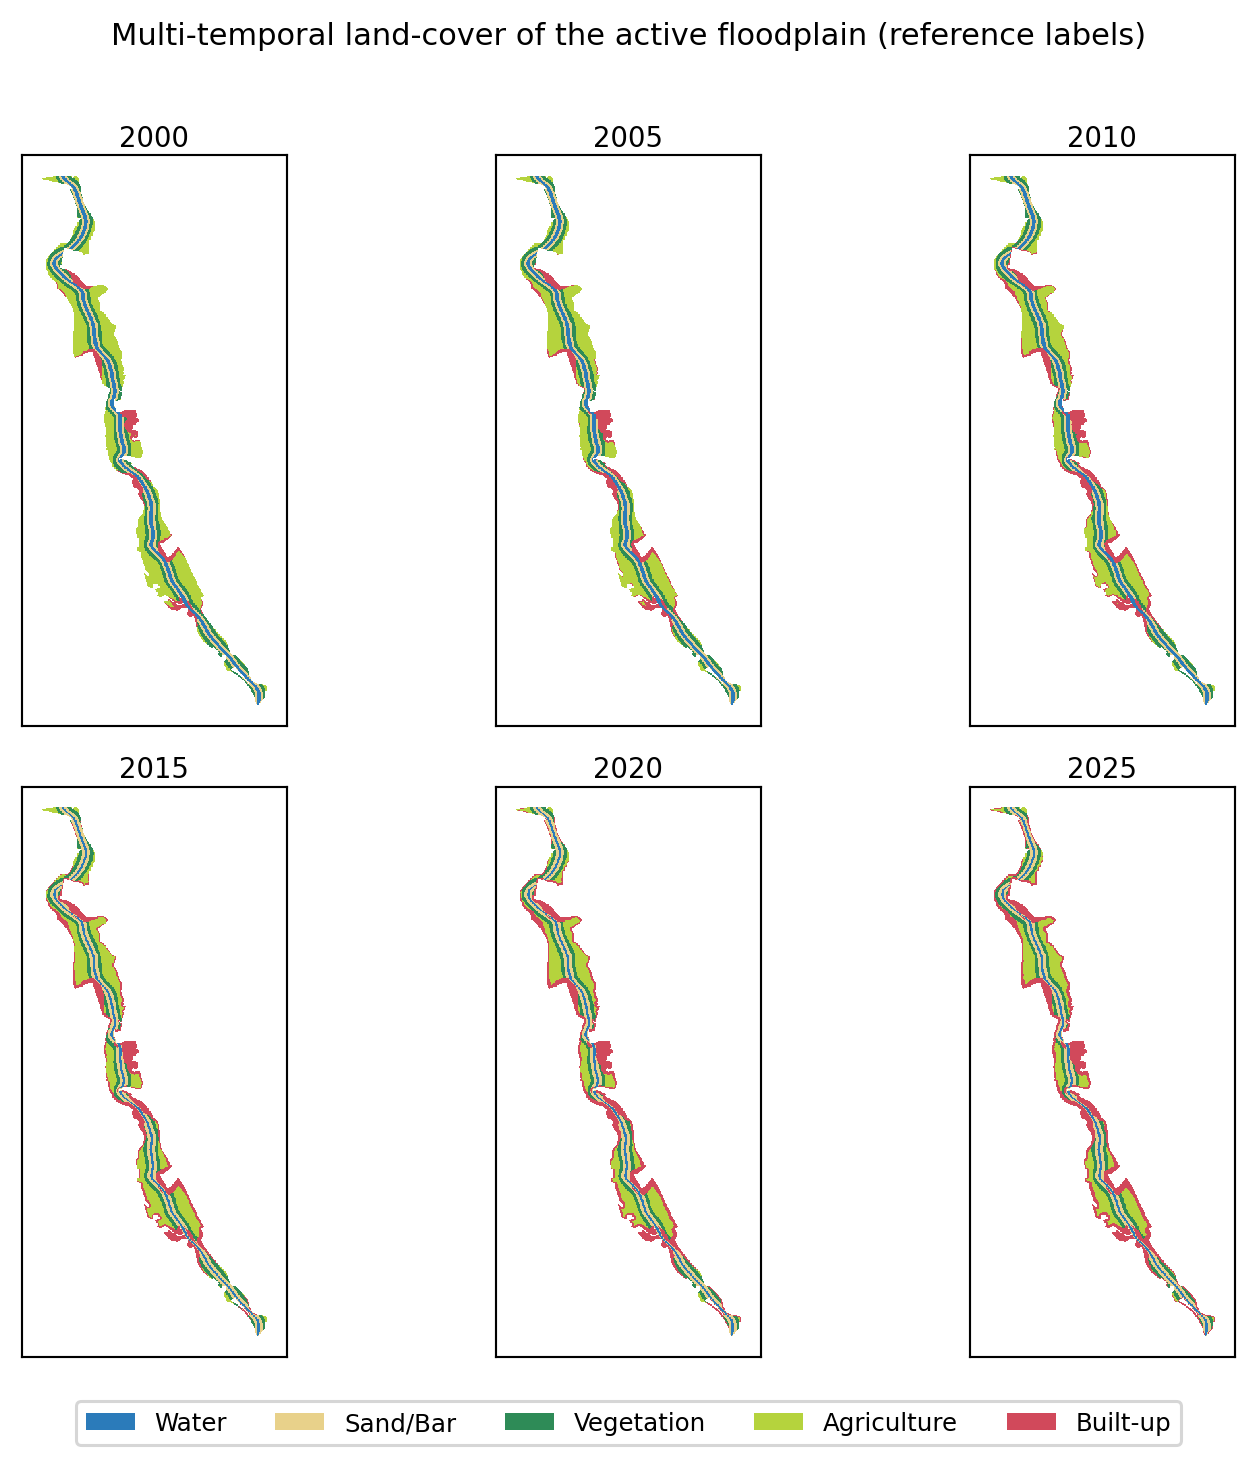
\includegraphics[width=\columnwidth]{fig2_multitemporal.png}
\caption{Multi-temporal reference land cover of the active floodplain, 2000 to 2025, showing progressive built-up expansion from the channel margins and interior nodes.}
\label{fig:multitemporal}
\end{figure}

\subsection{Feature engineering}
Each pixel is described by a 17-dimensional feature vector: the six reflectance bands; six spectral indices, namely NDVI \cite{rouse1974ndvi}, MNDWI \cite{xu2006mndwi}, NDWI \cite{mcfeeters1996ndwi}, NDBI \cite{zha2003ndbi}, SAVI \cite{huete1988savi}, and BSI \cite{rikimaru2002bsi}; four terrain descriptors (elevation, slope, HAND, distance-to-river); and a $3\times3$ NIR standard-deviation texture. The spectral indices target the physical contrasts of interest, water and moisture (MNDWI, NDWI), vegetation vigour (NDVI, SAVI), built-up and bare surfaces (NDBI, BSI), while terrain descriptors add non-spectral discrimination. Fig.~\ref{fig:inputs} shows representative inputs for 2025. Terrain features receive mild additive jitter so that a classifier cannot exploit fixed pixel positions as a proxy for identity.

\begin{figure}[!t]
\centering
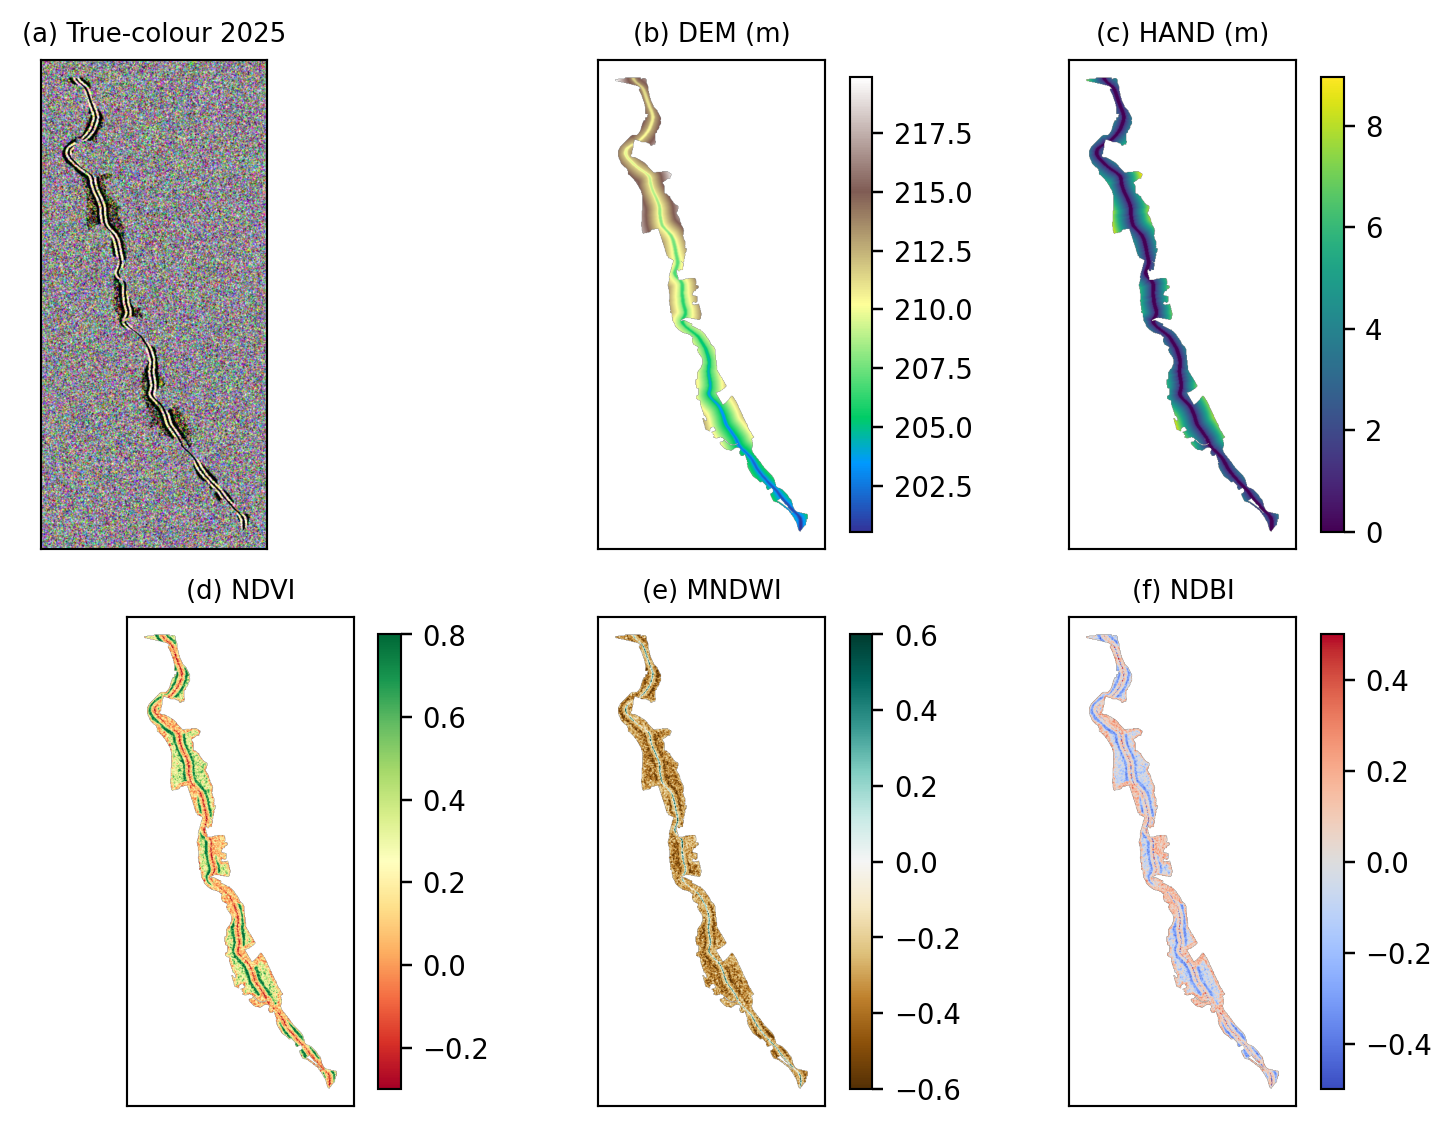
\includegraphics[width=\columnwidth]{fig3_inputs.png}
\caption{Representative model inputs for 2025: (a) true-colour composite, (b) DEM, (c) HAND, (d) NDVI, (e) MNDWI, (f) NDBI.}
\label{fig:inputs}
\end{figure}

\subsection{Evaluation protocol}
To prevent spatial autocorrelation from inflating accuracy, the analysis grid is partitioned by row: the northern 72\% (rows 0 to 599) supplies training reference pixels and the southern 28\% (rows 600 to 833) is an untouched spatial hold-out. A single stratified evaluation set of 39{,}832 pixels is drawn from the hold-out with equal allocation, up to 1{,}500 pixels per class and epoch, pooled across all six epochs, and every classifier, Random Forest, SVM, and CNN, is scored on these identical pixels. This guarantees a fair, leakage-controlled comparison across fundamentally different model families. Because the grid contains the floodplain and its urban surroundings, built-up reference pixels include extensive urban fabric outside the floodplain; these scores therefore measure five-class discrimination across the grid, and the accuracy of floodplain built-up area is assessed separately against the reference in Section~\ref{sec:change}. Accuracy is reported as overall accuracy, Cohen's $\kappa$ \cite{cohen1960kappa}, and macro-averaged F1, following standard practice in classification accuracy assessment \cite{congalton1991review,foody2002status}.

\subsection{Random Forest and SVM classifiers}
The Random Forest \cite{breiman2001random} uses 300 trees with balanced class weighting and a minimum leaf size of two, trained on 27{,}000 stratified pixels (900 per class per epoch) drawn only from the training region. An RBF support-vector machine \cite{cortes1995svm} ($C=10$, scale $\gamma$) is trained on a standardized 5{,}000-pixel subset as a kernel baseline. The trained Random Forest is applied wall-to-wall to every epoch to produce the operational land-cover time series (Fig.~\ref{fig:rfmaps}).

\subsection{Fully-convolutional neural network}
To test whether spatial context improves detection of sparse, edge-adjacent built-up, we implemented a compact fully-convolutional network \cite{long2015fully} independently in NumPy. The architecture is
\[
\text{Conv}_{3\times3}(9{\to}24)\text{--ReLU--}\text{Conv}_{3\times3}(24{\to}32)\text{--ReLU--}
\]
\[
\text{Conv}_{3\times3}(32{\to}32)\text{--ReLU--}\text{Conv}_{1\times1}(32{\to}5),
\]
giving a $7\times7$ receptive field over a nine-channel input (six bands plus NDVI, MNDWI, NDBI). Training uses pixel-wise softmax cross-entropy and the Adam optimizer \cite{kingma2015adam}. The convolution's backward pass was verified against central-difference numerical gradients (maximum relative error below $2\times10^{-8}$). Training tiles ($48\times48$) are extracted only from the northern region; the network is then scored on the same hold-out pixels as the other models and applied wall-to-wall by overlap-averaging tile softmax outputs.

Concretely, a tile enters as nine co-registered channels; the three $3\times3$ layers lift the representation at every cell to 24 and then 32 channels while widening its spatial support to $7\times7$ cells, a $350\times350$~m window of 12.25~ha on the 50~m grid, and the closing $1\times1$ layer maps those 32 channels to the five class scores, for 1{,}968, 6{,}944, 9{,}248, and 165 weights, 18{,}325 in total. A narrow built-up parcel on the floodplain margin is therefore scored together with its 12.25~ha neighbourhood rather than in isolation, which is why the CNN reaches a built-up IoU of 0.939 and matches the 2025 reference area to within 1\%, where the pixel-wise Random Forest under-detects it by about 30\% (Section~\ref{sec:results}).

\begin{algorithm}[!t]
\caption{Land-cover classification and encroachment mapping}
\label{alg:classify}
\begin{algorithmic}[1]
\Require reflectance epochs $\{R_y\}$; terrain layers (DEM, slope, HAND, $d_{\mathrm{riv}}$); floodplain mask $M$; cell size $\rho$
\Ensure LULC maps $\{L_y\}$; encroachment areas $\{A_y\}$; transition matrix $T$
\For{each epoch $y$}
  \State compute NDVI, MNDWI, NDWI, NDBI, SAVI, BSI from $R_y$
  \State stack $F_y$: 6 bands, 6 indices, DEM, slope, HAND, $d_{\mathrm{riv}}$, texture \Comment{17-D}
\EndFor
\State split rows into north (train) and south (test) blocks
\State draw balanced pixels from north; train RF and SVM; train CNN on north tiles
\State score RF, SVM, CNN on the shared south hold-out (OA, $\kappa$, F1, IoU)
\For{each epoch $y$}
  \State $L_y \gets \mathrm{RF}(F_y)$ \Comment{wall-to-wall operational map}
  \State $A_y \gets \rho^2 \, \lvert \{L_y=\text{Built-up}\} \cap M \rvert$
\EndFor
\State $T \gets$ 5$\times$5 class transitions from $L_{2000},L_{2025}$ within $M$
\end{algorithmic}
\end{algorithm}
\subsection{Change detection and encroachment}

Land-cover change is quantified by post-classification comparison \cite{singh1989digital,lu2004change} of the Random Forest maps. We compute the full $5\times5$ class-transition matrix between 2000 and 2025 within the floodplain, the per-epoch class areas, and the built-up (encroachment) trajectory as both absolute area and percentage of floodplain area.

\subsection{Forecasting}
\emph{Areal.} Three growth models, linear, exponential, and logistic, are fitted to the 2000 to 2025 encroachment series by nonlinear least squares. The logistic form
\begin{equation}
A(t)=\frac{K}{1+\exp\!\big(-r\,(t-t_0)\big)}
\label{eq:logistic}
\end{equation}
represents saturating growth bounded by the finite floodplain; such parametric trend models are standard in applied time-series forecasting \cite{box2015time,hyndman2018forecasting}. The lowest-RMSE model is used to forecast 2030 and 2035, with a 90\% interval from a 2000-sample residual bootstrap.

Concretely, fitting \eqref{eq:logistic} to the six mapped areas returns $K=22.02$~km\textsuperscript{2}, $r=0.0950\,\text{yr}^{-1}$, and $t_0=2013.6$, so $A(2030)=22.02/\big(1+e^{-0.0950\times16.4}\big)=18.2$~km\textsuperscript{2} and $A(2035)=19.5$~km\textsuperscript{2}. These areas are what the spatial stage consumes: with $A_{2025}=16.41$~km\textsuperscript{2} and $\rho=50$~m, the cell demand $(\hat{A}(h)-A_{2025})/\rho^{2}$ of Algorithm~\ref{alg:forecast} is $(18.2-16.41)/0.0025=716$ cells of 0.25~ha for 2030, allocated to the 716 highest-suitability open floodplain cells, and a further 520 cells for 2035 after the drivers are recomputed. The carrying capacity thus caps the demand the allocation model can ever be asked to place.

\emph{Spatial.} A logistic suitability model is trained on the 2015 to 2025 conversions mapped by the Random Forest using five physical drivers, distance to existing built-up, distance to river, HAND, distance to urban edge, and $5\times5$ neighbourhood built-up density, and applied in a cellular-automata manner \cite{yang2014markov,verburg2002clue}: the areal-model demand for each horizon is allocated to the highest-suitability open floodplain cells, first to 2030 and then, updating the drivers, to 2035.

\emph{Validation.} A hindcast trains the identical driver model on the 2000 to 2015 conversion and allocates the 2015 to 2025 demand mapped by the Random Forest; the prediction is compared with the 2025 Random Forest map using built-up cell agreement over the floodplain and the Figure of Merit \cite{pontius2008comparing}, $\text{FoM}=\text{hits}/(\text{hits}+\text{misses}+\text{false alarms})$, computed on the changed cells.

\begin{algorithm}[!t]
\caption{Cellular-automata encroachment forecasting}
\label{alg:forecast}
\begin{algorithmic}[1]
\Require built-up series $\{A_y\}$; drivers $D$; floodplain mask $M$; horizons $\mathcal{H}=\{2030,2035\}$; cell size $\rho$
\Ensure projected built-up masks $\{B_h\}$
\State fit linear, exponential, and logistic $A(t)$; keep lowest-RMSE model $\hat{A}$
\State train logistic suitability $S$ on mapped 2015-to-2025 conversions using $D$
\State $B \gets \{L_{2025}=\text{Built-up}\} \cap M$
\For{$h \in \mathcal{H}$ in ascending order}
  \State $n_h \gets \max\!\big(0,\ (\hat{A}(h)-A_{2025})/\rho^2\big)$ \Comment{cell demand}
  \State rank open floodplain cells of $M\setminus B$ by $S$; convert top $n_h$ to built-up
  \State $B_h \gets B$; recompute drivers $D$ from $B_h$
\EndFor
\end{algorithmic}
\end{algorithm}

\section{Results}\label{sec:results}

\subsection{Classification accuracy}
Table~\ref{tab:models} reports the three classifiers on the shared spatial hold-out (Fig.~\ref{fig:modelcomp}). The Random Forest reaches 0.947 overall accuracy ($\kappa=0.933$) and the support-vector machine 0.945 ($\kappa=0.931$). The fully-convolutional network attains the best scores, 0.957 overall accuracy and $\kappa=0.946$, its spatial context supplying information that the pixel-wise classifiers lack.

\begin{table}[!t]
\caption{Classifier performance on the shared spatial-hold-out test set (39{,}832 pixels, pooled over six epochs).}
\label{tab:models}
\centering
\begin{tabular}{lccc}
\toprule
Model & Overall Acc. & Cohen $\kappa$ & Macro-F1 \\
\midrule
Random Forest (300 trees) & 0.9471 & 0.9334 & 0.9514 \\
SVM (RBF, $C{=}10$) & 0.9449 & 0.9307 & 0.9490 \\
CNN (fully-convolutional) & \textbf{0.9572} & \textbf{0.9462} & \textbf{0.9593} \\
\bottomrule
\end{tabular}
\end{table}

Per-class results explain the ranking. For the Random Forest, Water is near-perfect (F1~0.999) and Built-up is strong (F1~0.971), while Agriculture is hardest (F1~0.888), confused chiefly with vegetation and, to a lesser extent, with sand/bar and built-up surfaces, a realistic difficulty given their spectral similarity. The confusion matrix and Gini feature importance are shown in Fig.~\ref{fig:rfcm}: NIR reflectance, HAND, and SAVI are the most informative features, confirming that the hydrological terrain descriptor contributes materially alongside spectral information. The CNN's per-class Intersection-over-Union (Fig.~\ref{fig:cnn}) is highest for Built-up and Water (0.939 and 0.974) and lowest for Agriculture (0.878), mirroring the same spectral confusion but recovering built-up parcels more completely through context.

\begin{figure}[!t]
\centering
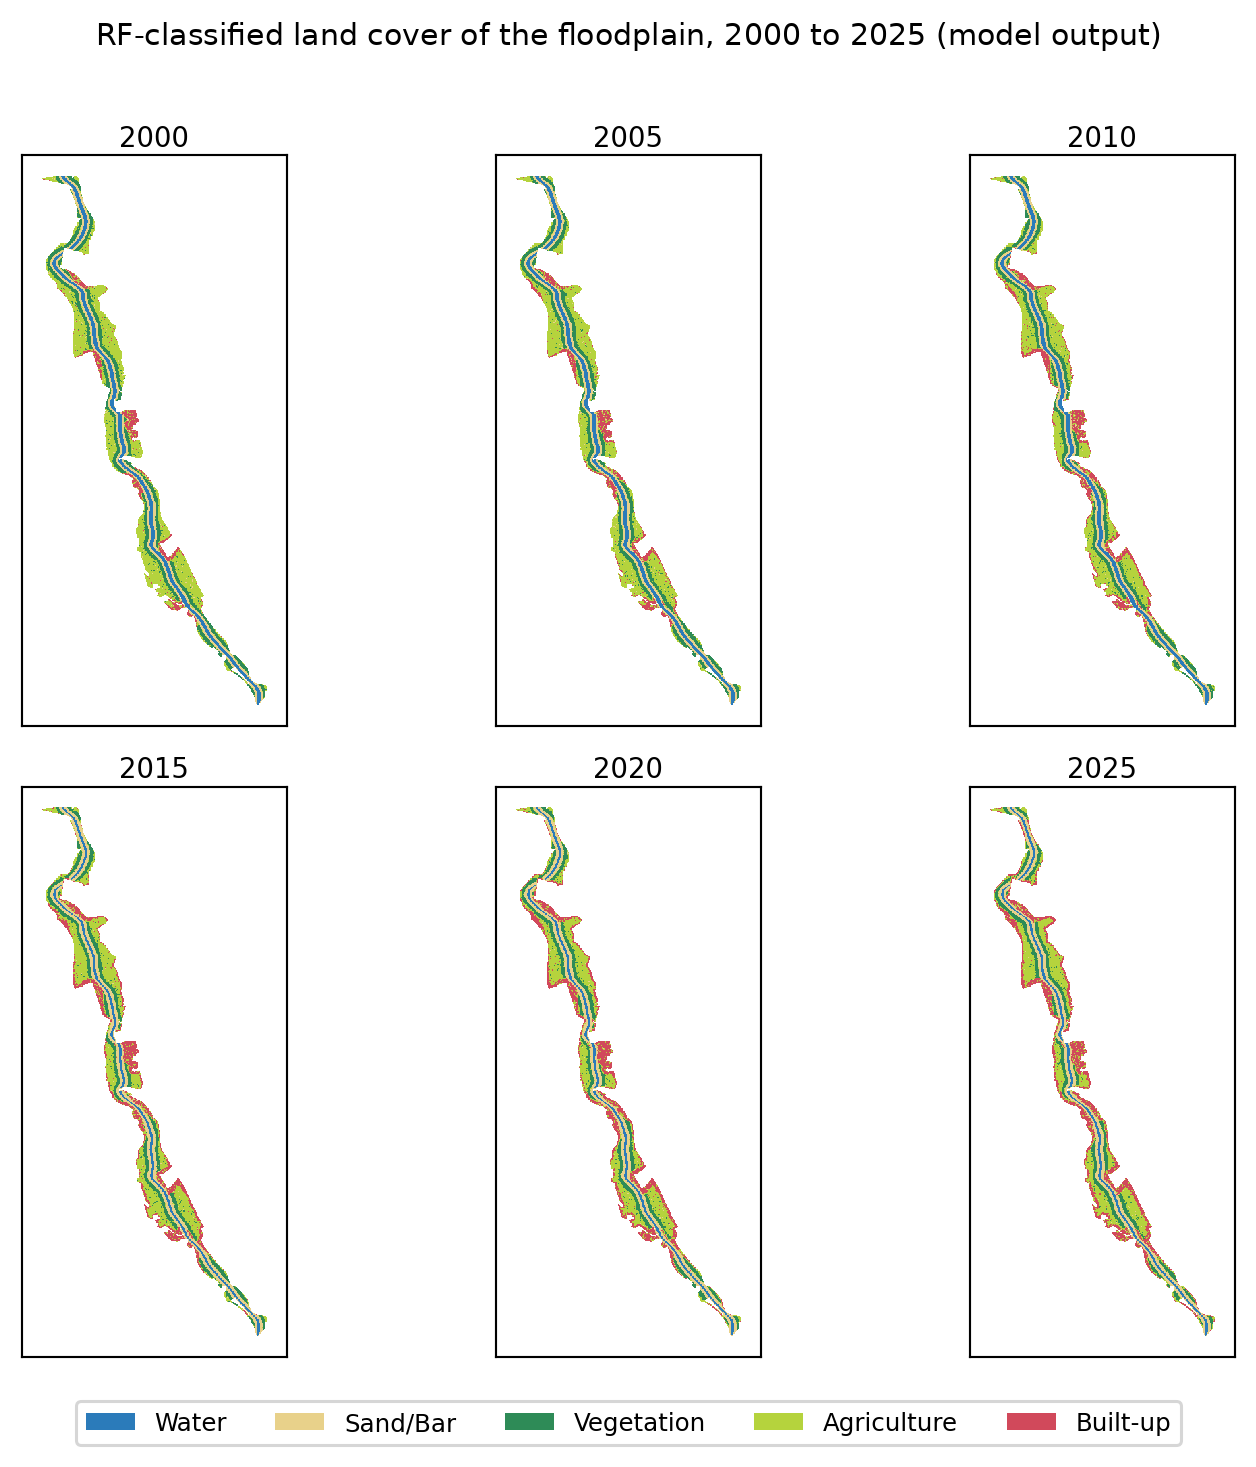
\includegraphics[width=\columnwidth]{fig12_rf_maps.png}
\caption{Random Forest wall-to-wall land-cover classification of the floodplain, 2000 to 2025, the operational model output used for change detection and forecasting.}
\label{fig:rfmaps}
\end{figure}

\begin{figure}[!t]
\centering
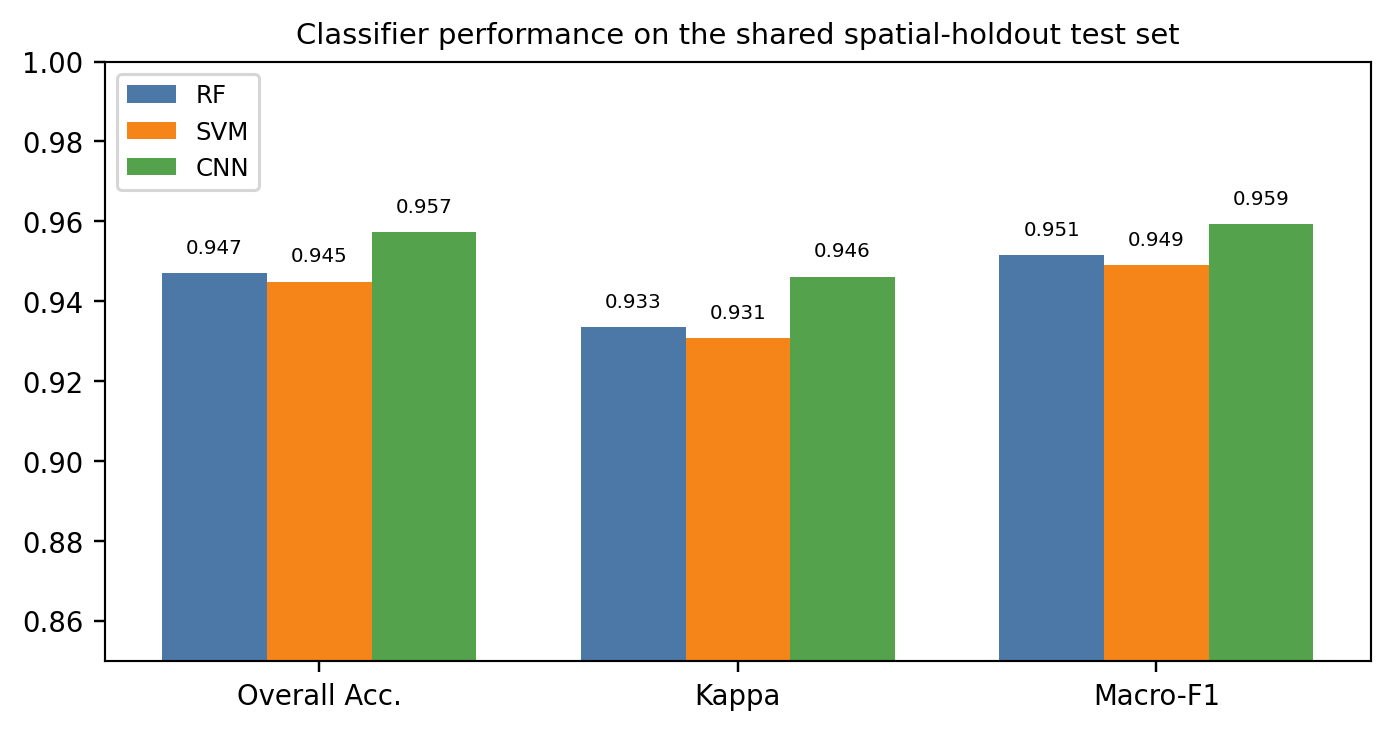
\includegraphics[width=\columnwidth]{fig5_modelcomp.png}
\caption{Overall accuracy, Cohen $\kappa$, and macro-F1 for the three classifiers on the identical spatial-hold-out test set.}
\label{fig:modelcomp}
\end{figure}

\begin{figure}[!t]
\centering
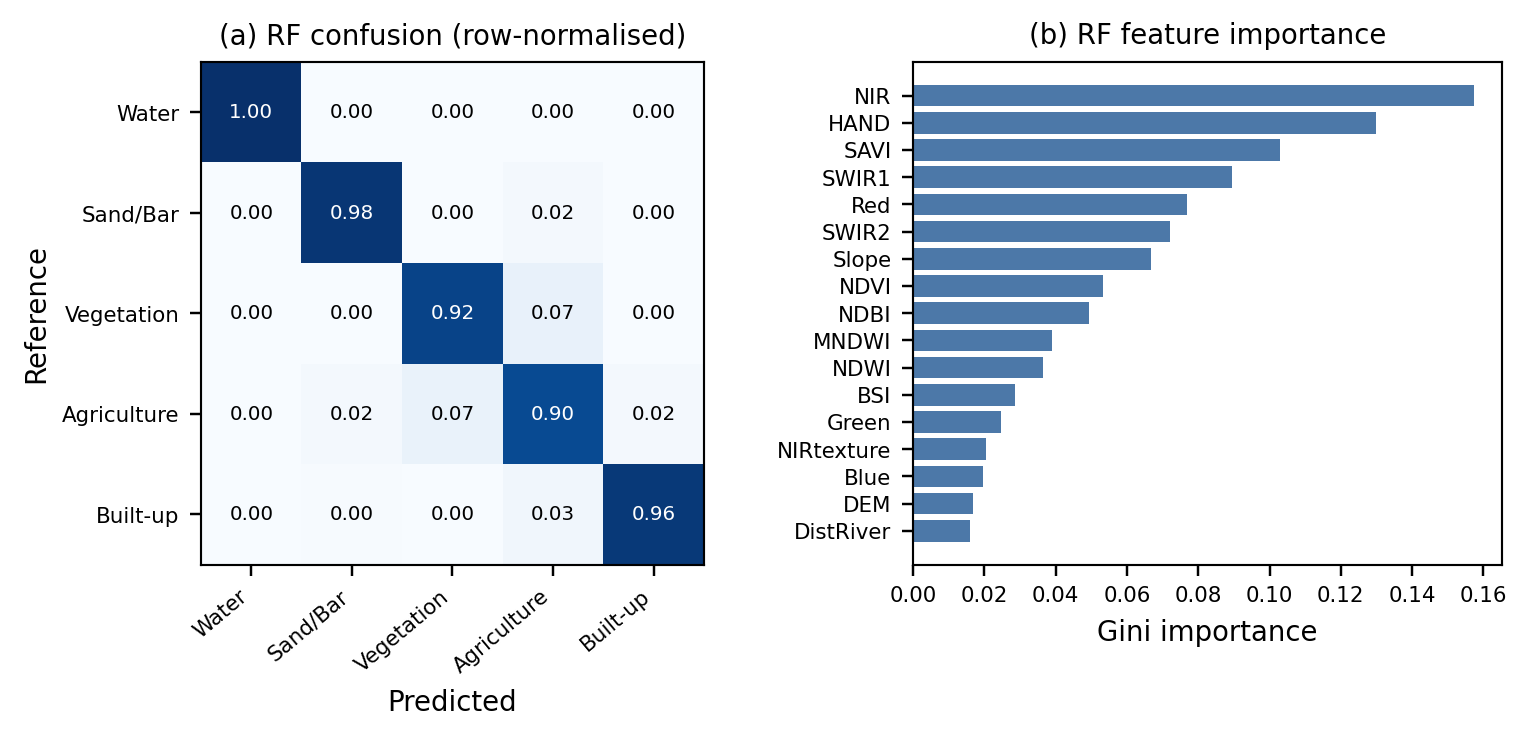
\includegraphics[width=\columnwidth]{fig4_rf_cm_fi.png}
\caption{(a) Row-normalized Random Forest confusion matrix on the shared hold-out; (b) Gini feature importance. Agriculture--vegetation confusion dominates residual error; NIR, HAND, and SAVI are the most important features.}
\label{fig:rfcm}
\end{figure}


\begin{figure}[!t]
\centering
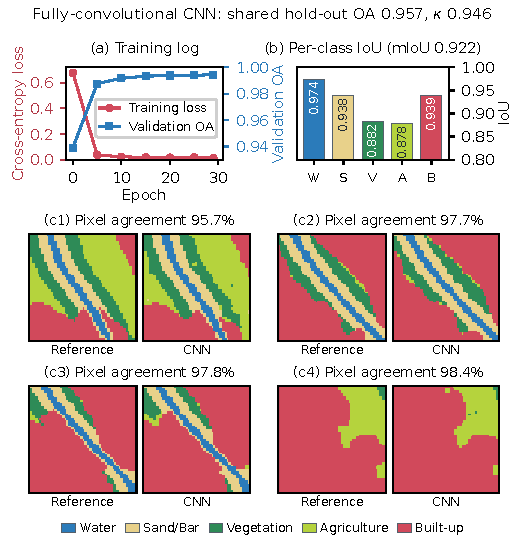
\includegraphics[width=0.97\columnwidth]{fig6_cnn.pdf}
\caption{Fully-convolutional CNN. (a) Training loss and validation overall accuracy (OA) on held-out northern tiles, logged every five epochs. (b) Per-class IoU on the shared hold-out (W: water, S: sand/bar, V: vegetation, A: agriculture, B: built-up). (c1) to (c4) Example $48\times48$ tiles from the southern spatial hold-out, reference (left) and CNN prediction (right), with per-tile pixel agreement.}
\label{fig:cnn}
\end{figure}

\subsection{Land-cover change and encroachment}\label{sec:change}
Table~\ref{tab:areas} and Fig.~\ref{fig:areas} summarize floodplain land-cover composition over 2000 to 2025 from the Random Forest maps. Built-up area within the floodplain rises monotonically from 4.82~km\textsuperscript{2} (6.7\% of the floodplain) in 2000 to 16.41~km\textsuperscript{2} (22.9\%) in 2025, an increase of roughly 240\%. This expansion is drawn primarily from agriculture, which declines from 26.3 to 20.5~km\textsuperscript{2}, and secondarily from vegetation; open water does not convert directly to built-up land, and its decline reflects conversion to sand and bar surfaces. The full 2000 to 2025 transition matrix (Fig.~\ref{fig:transition}) makes the pathways explicit: the largest built-up gains come from agricultural (8.83~km\textsuperscript{2}) and vegetated (2.61~km\textsuperscript{2}) land, consistent with peripheral agricultural parcels being the first to be converted.

Because the benchmark labels are exact, these mapped areas can be checked against the reference. The reference contains 6.72~km\textsuperscript{2} (9.4\%) of built-up land in 2000 and 23.51~km\textsuperscript{2} (32.8\%) in 2025, so the Random Forest maps under-detect floodplain built-up by about 30\% in 2025, whereas the CNN maps contain 7.23 and 23.70~km\textsuperscript{2}, within 1\% of the reference in 2025. The Random Forest trajectory used below for change detection and forecasting is therefore a conservative estimate of encroachment; the closer agreement of the CNN is consistent with its use of spatial context.

\begin{table}[!t]
\caption{Floodplain land-cover area by epoch (km\textsuperscript{2}), from Random Forest maps. Floodplain area 71.8~km\textsuperscript{2}.}
\label{tab:areas}
\centering
\small
\begin{tabular}{lcccccc}
\toprule
Class & 2000 & 2005 & 2010 & 2015 & 2020 & 2025 \\
\midrule
Water        & 10.75 & 10.76 & 10.84 & 6.73 & 6.73 & 6.74 \\
Sand/Bar     & 13.31 & 13.00 & 12.63 & 16.27 & 16.24 & 15.88 \\
Vegetation   & 16.61 & 15.96 & 14.85 & 14.03 & 13.13 & 12.22 \\
Agriculture  & 26.28 & 25.25 & 24.51 & 22.87 & 21.32 & 20.52 \\
Built-up     & 4.82 & 6.80 & 8.95 & 11.87 & 14.35 & 16.41 \\
\midrule
Built-up (\%) & 6.7 & 9.5 & 12.5 & 16.5 & 20.0 & 22.9 \\
\bottomrule
\end{tabular}
\end{table}

\begin{figure}[!t]
\centering
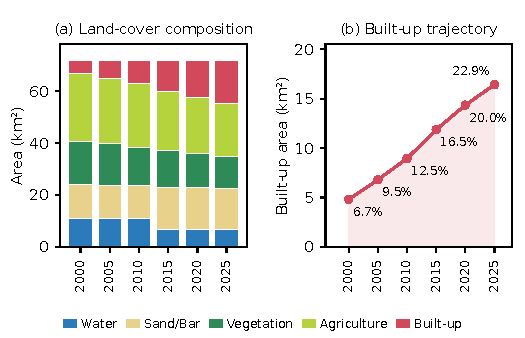
\includegraphics[width=\columnwidth]{fig7_areas.pdf}
\caption{Random Forest maps, 2000 to 2025: (a) floodplain land-cover composition and (b) built-up area, labelled with its share of the floodplain.}
\label{fig:areas}
\end{figure}

\begin{figure}[!t]
\centering
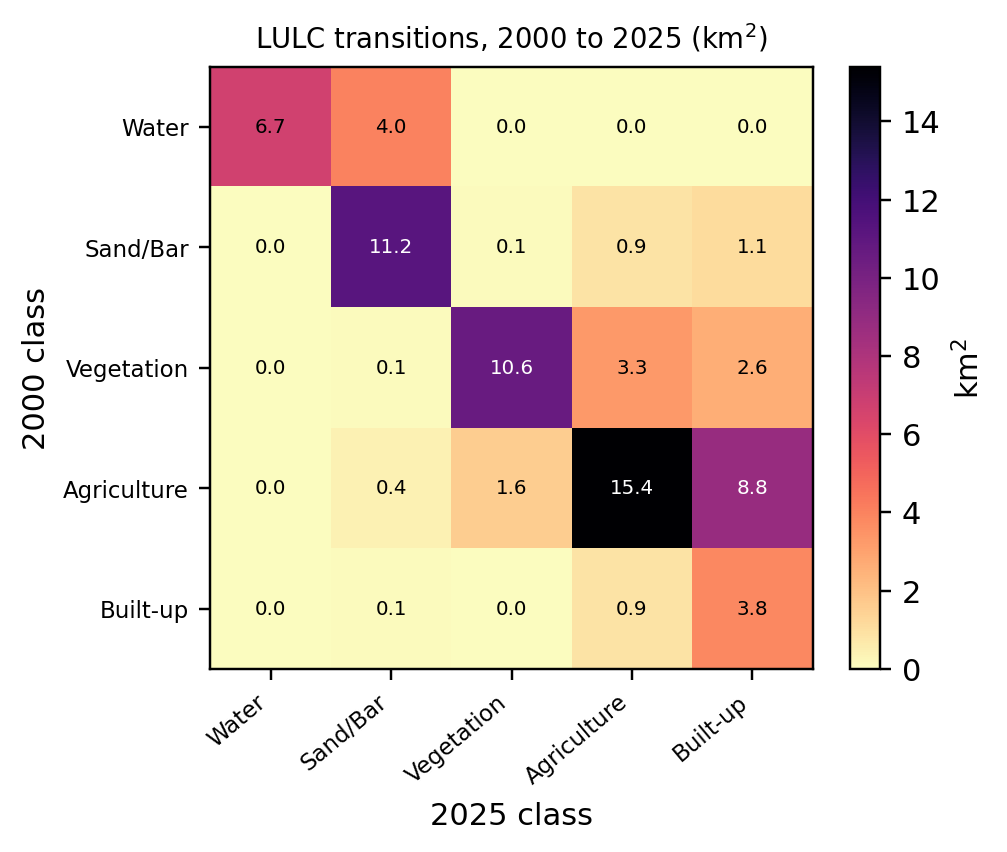
\includegraphics[width=0.82\columnwidth]{fig8_transition.png}
\caption{Land-cover transition matrix within the floodplain, 2000 to 2025 (km\textsuperscript{2}). Built-up gains derive mainly from agriculture and vegetation.}
\label{fig:transition}
\end{figure}

\subsection{Forecasting and validation}
Among the growth models the logistic form fits best (RMSE 0.110~km\textsuperscript{2}, versus 0.222 exponential and 0.234 linear), with estimated carrying capacity $K=22.0$~km\textsuperscript{2}, rate $r=0.095\,\text{yr}^{-1}$, and inflection near 2014. It projects floodplain built-up of 18.2~km\textsuperscript{2} (25.4\%) by 2030 and 19.5~km\textsuperscript{2} (27.1\%) by 2035, with 90\% bootstrap bands of $[17.8,18.5]$ and $[18.9,20.0]$~km\textsuperscript{2} respectively (Fig.~\ref{fig:forecast}). We emphasize that the logistic model infers proximity to saturation from only six observations, so its carrying capacity is weakly constrained; the near-flattening of the forecast should be read as one plausible bounded-growth scenario rather than a settled prediction, and the three fitted curves in Fig.~\ref{fig:forecast} bracket the areal uncertainty.

The driver-based spatial model translates this demand into maps. Fig.~\ref{fig:future} shows the learned encroachment-suitability surface and the projected 2030 and 2035 built-up footprints, with newly-converted cells concentrated along the inner floodplain margins and around existing development, as the suitability drivers imply.

The spatial model's credibility rests on the hindcast (Fig.~\ref{fig:hindcast}). Trained on 2000 to 2015 conversions and asked to allocate the mapped 2015 to 2025 demand, it reproduces the 2025 built-up pattern of the Random Forest maps with 87.1\% cell agreement over the floodplain and a Figure of Merit of 0.492 on the changed cells (3{,}189 hits, 1{,}846 misses, 1{,}445 false alarms). For context, in a comparison of 13 applications of nine land-change models, the error exceeded the correctly predicted change, implying a Figure of Merit below 0.5, in 12 of the 13 applications \cite{pontius2008comparing}, and a recent heuristic cellular-automata model reports a validation Figure of Merit of 37.64\% \cite{tang2024urban}. The hindcast value of 0.492 indicates that the driver set captures much of the spatial logic of encroachment in the benchmark; because those drivers are known by construction, it should not be read as the accuracy expected on real imagery.

\begin{figure}[!t]
\centering
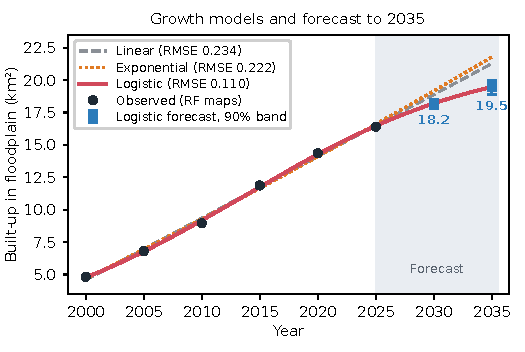
\includegraphics[width=\columnwidth]{fig9_forecast.pdf}
\caption{Growth models fitted to the 2000 to 2025 built-up series of the Random Forest maps, and the logistic forecast to 2035 with its 90\% bootstrap band. The logistic model has the lowest RMSE.}
\label{fig:forecast}
\end{figure}

\begin{figure}[!t]
\centering
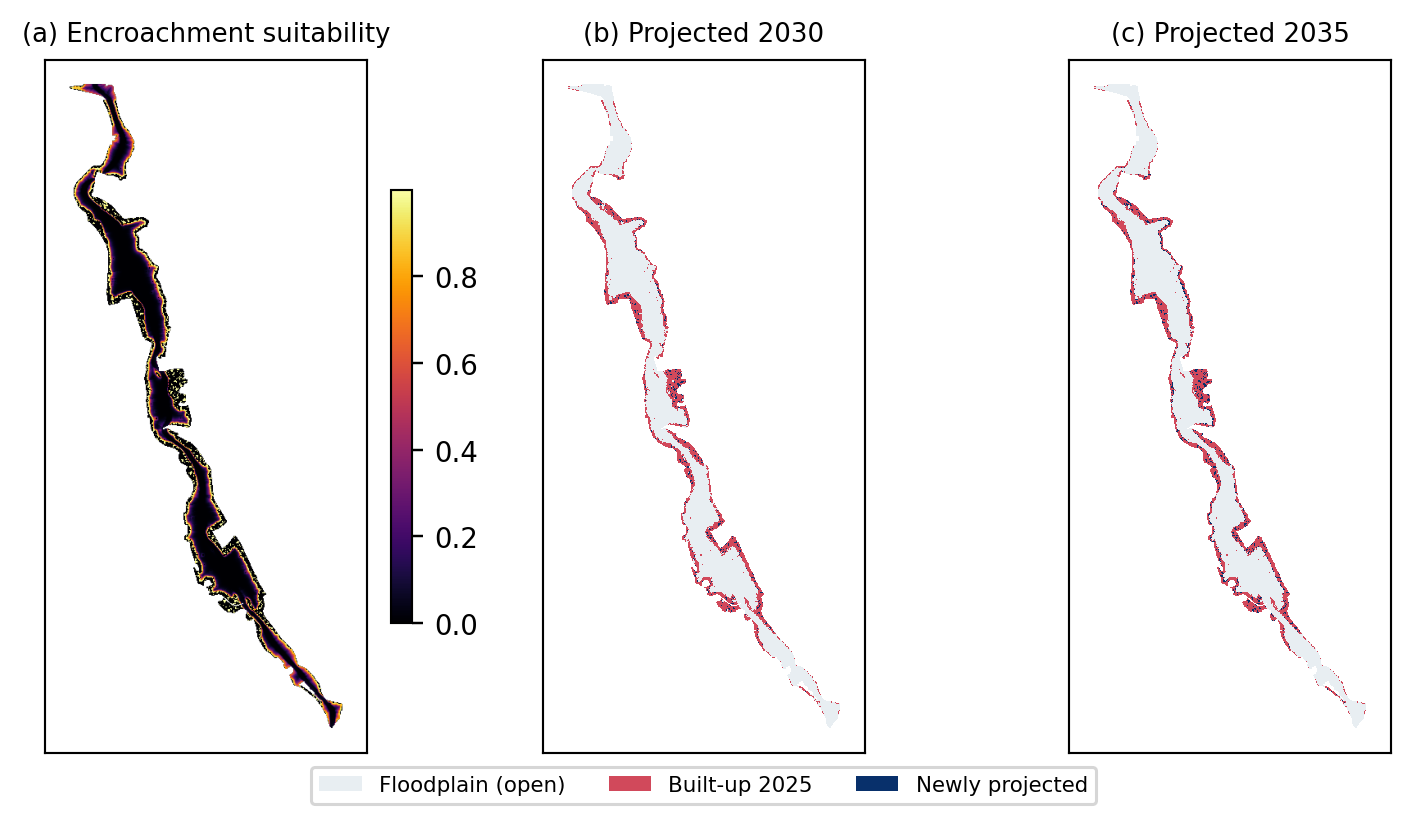
\includegraphics[width=\columnwidth]{fig10_future.png}
\caption{(a) Learned encroachment-suitability surface; (b) projected 2030 and (c) 2035 built-up, with newly-converted floodplain cells highlighted.}
\label{fig:future}
\end{figure}

\begin{figure}[!t]
\centering
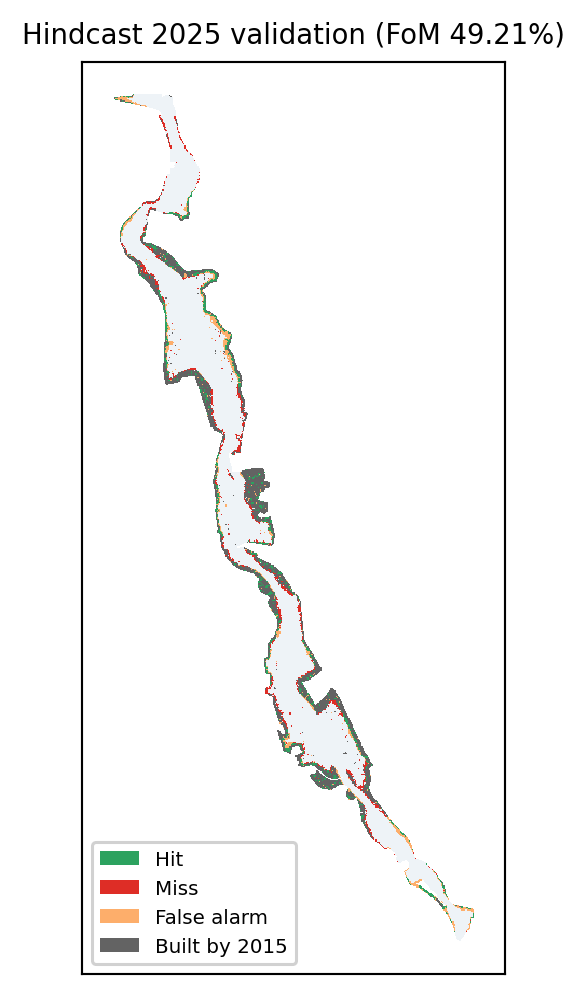
\includegraphics[width=0.66\columnwidth]{fig11_hindcast.png}
\caption{Hindcast validation: the driver model trained on 2000 to 2015 conversions allocates the 2015 to 2025 demand of the Random Forest maps and is compared with the 2025 Random Forest map (Figure of Merit 0.49).}
\label{fig:hindcast}
\end{figure}

\section{Discussion}\label{sec:discussion}
Three findings stand out. First, terrain descriptors, and HAND in particular, are among the most informative features. In this benchmark that is partly by construction, because the encroachment-pressure field favours the floodplain margins, but it shows that the pipeline can exploit hydrological terrain information that purely spectral classifiers discard; whether the same holds on real imagery remains to be tested. Second, spatial context measurably helps: beyond its higher hold-out accuracy, the CNN's floodplain built-up area agrees with the reference to within 1\% in 2025, whereas the pixel-wise Random Forest under-detects it by about 30\%, and floodplain encroachment monitoring depends on exactly this sensitivity. Third, within the benchmark the spatial forecasting model generalizes across time in the hindcast, suggesting that the drivers, proximity to existing development, the river, and the urban edge, together with local elevation, encode a transferable mechanism rather than an epoch-specific pattern.

Table~\ref{tab:related} places these results beside published studies, and the comparison must respect what each number measures. The classification accuracies obtained here (94.7\% for the Random Forest and 95.7\% for the CNN) use exact, noise-free labels, which removes the annotation error and mixed-pixel ambiguity that lower accuracy on real scenes; they characterize the ceiling of the method under clean supervision rather than field performance. Simulation agreement is a separate quantity: validations of Delhi growth models report 79.78\% overall accuracy for a CA--ANN simulation \cite{jain2024future}, 95.62\% for a cellular-automata simulation of built-up extent \cite{tripathy2019monitoring}, and 98.63\% for a Land Change Modeler simulation \cite{singh2022land}, against 87.1\% cell agreement in the hindcast here. Because overall agreement also counts cells that do not change, the Figure of Merit, computed over observed and predicted change only, is the more discriminating measure \cite{pontius2008comparing}. The value of these comparisons lies not in the absolute margins but in confirming that the feature design, the shared spatial hold-out, and the driver set behave as intended, so that the same models can be re-scored on operational imagery, where more modest accuracies should be expected.

The principal limitation is the data-provenance constraint discussed above: the imagery is a controlled benchmark, not observed reflectance, so the absolute encroachment figures characterize the model--benchmark system rather than the physical river. This is also a methodological strength for validation, because ground truth is exact, but operational conclusions about the actual Yamuna require real imagery. In addition, change detection and forecasting here use the Random Forest maps, which under-detect floodplain built-up relative to the reference; driving the same stages with the CNN maps would raise the encroachment estimates. Because the pipeline ingests analysis-ready reflectance unchanged, that substitution is direct: multi-date Landsat \cite{wulder2019current} and Sentinel-2 \cite{drusch2012sentinel} composites from Google Earth Engine \cite{gorelick2017gee}, with historical labels from surveyed or high-resolution reference data, would drive the identical classification, change-detection, and forecasting stages. Further work includes temporal models such as continuous change detection \cite{zhu2014continuous} and deeper encoder--decoder segmentation \cite{ronneberger2015unet} when dense training labels are available, and richer socio-physical drivers for the allocation model.

\section{Conclusion and Future Work}\label{sec:conclusion}
We presented a complete, reproducible AI framework for monitoring and forecasting built-up encroachment on the Delhi Yamuna floodplain, built on the river's real digitized active-floodplain geometry and evaluated under a strict spatial hold-out shared by all models. Random Forest and an independently implemented fully-convolutional CNN classify land cover on the shared spatial hold-out at 0.947 and 0.957 overall accuracy respectively; post-classification analysis of the Random Forest maps shows floodplain built-up rising from 6.7\% to 22.9\% between 2000 and 2025, a conservative estimate that the CNN maps bring to within 1\% of the 2025 reference; and a logistic areal model coupled to a driver-based cellular-automata allocation projects the trajectory and its spatial footprint to 2035, with a hindcast Figure of Merit of 0.49 supporting the spatial model. The framework is engineered for direct transfer to operational Landsat and Sentinel-2 imagery, offering planning authorities a transparent tool, validated here on a controlled benchmark, for tracking and anticipating floodplain encroachment. Building on the accuracy established here, future work will exercise the same pipeline unchanged on multi-date Landsat and Sentinel-2 composites of this reach, drive the change-detection and allocation stages from the CNN maps whose areas match the reference most closely, and extend the driver set with regulatory and socio-economic layers, so that the framework reports encroachment for the physical river at the resolution and cadence that enforcement requires.

\section*{Reproducibility}
The complete pipeline, from the floodplain polygon through every reported figure and metric, is implemented as a single executed notebook. The implementation uses NumPy \cite{harris2020array} for array computation and the terrain, forecasting, and neural-network components, and scikit-learn \cite{pedregosa2011scikit} for the Random Forest and support-vector classifiers. Random seeds are fixed throughout, so all results are deterministic and reproducible.

\bibliographystyle{IEEEtran}
\bibliography{refs}

\end{document}
